\chapter{Architecture}

Here is the main class diagram, it only represents the frame of the API:
\begin{figure}[H]
\begin{center}
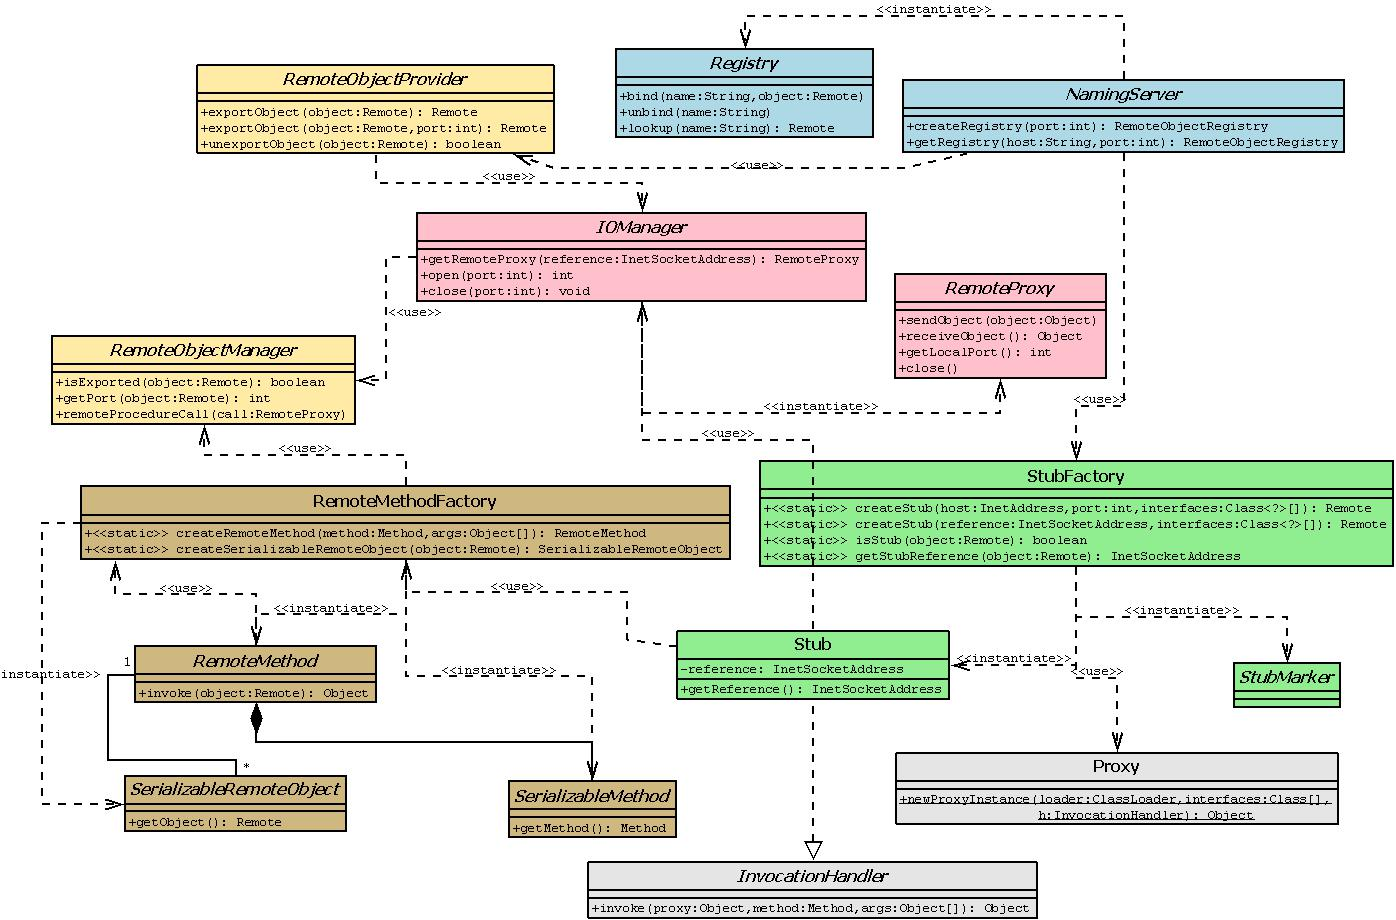
\includegraphics[scale=0.42,angle=90]{../img/diag_classes.jpeg}
\caption{UML class diagram}
\end{center}
\end{figure}
\medskip
\hspace{-.6cm}You can see clearly five different parts:
\begin{itemize}
\item Naming server
\item Object sharing
\item Communication layer
\item Distant calls
\item Stub
\end{itemize}
\medskip
We identify an object shared on the network by an IP address and the port used to receive distant calls.

\section{Naming server}
The registry provider provide a stub when asked to a distant register.

\section{Object sharing}
The RemoteObjectManager interface is inner the API, it should not be used by the end-user. It permit the distant call factory to check if the object named in the parameters or returned value are exported, and if it's not the case, to obtain the port which is listened. It allows to the communication layer to pass a distant call to a shared object.

\section{Communication layer}
The RemoteProxy interface is encapsulate a socket, provided by an IOManager which has to open, start listen to, and close ports.

\section{Stub}
Thanks to the Java.reflect API, stubs are created dynamically, on-the-fly.

\section{Distant calls}
A RemoteMethod instance has to be serializable and has to contain all the parameters needed to the execution of the distant method on the shared object used in parameter.

